%%% Exemplo de utilizacao da classe ITA
%%%
%%%   por        Fabio Fagundes Silveira   -  ffs [at] ita [dot] br
%%%              Benedito C. O. Maciel     -  bcmaciel [at] ita [dot] br
%%%              Giovani Volnei Meinertz   -  giovani [at] ita [dot] br
%%%    	         Hudson Alberto Bode       -  bode [at] ita [dot]br
%%%    	         P. I. Braga de Queiroz    -  pi [at] ita [dot] br
%%%    	         Jorge A. B. Gripp         -  gripp [at] ita [dot] br
%%%    	         Juliano Monte-Mor         -  jamontemor [at] yahoo [dot] com [dot] br
%%%    	         Tarcisio A. B. Gripp      -  tarcisio.gripp [at] gmail [dot] com
%%%    	         
%%%
%%%  IMPORTANTE: O texto contido neste exemplo nao significa absolutamente nada.  :-)
%%%              respectivas utilizacoes.
%%%
%%%  Tese.tex  2016-08-25
%%%  HeadURL: http://www.apgita.org.br/apgita/teses-e-latex.php
%%%
%%% ITALUS
%%% Instituto Tecnologico de Aeronautica --- ITA, Sao Jose dos Campos, Brasil
%%%                   http://groups.yahoo.com/group/italus/
%%% Discussion list: italus {at} yahoogroups.com
%%%
%++++++++++++++++++++++++++++++++++++++++++++++++++++++++++++++++++++++++++++++
% Para alterar o TIPO DE DOCUMENTO, preencher a linha abaixo \documentclass[?]{?}
%   \documentclass[tg]{ita}			= Trabalho de Graduacao
%   \documentclass[tgfem]{ita}	= Para Engenheiras
%   								msc     		= Dissertacao de Mestrado
%   								mscfem   		= Para Mestras
%   								dsc      		= Tese de Doutorado
%   								dscfem   		= Para Doutoras
%   								quali    		= Exame de Qualificacao
%   								qualifem 		= Exame de Qualificacao para Doutoras
% Para 'Draft Version'/'Versao Preliminar' com data no rodape, adicionar 'dv':
%   \documentclass[dsc, dv]{ita} 
% Para trabalhos em Ingles, adicionar 'eng':
%   \documentclass[dsc, eng]{ita}
%		\documentclass[dsc, eng, dv]{ita}
%++++++++++++++++++++++++++++++++++++++++++++++++++++++++++++++++++++++++++++++
\documentclass[tg, eng]{ita}    % ITA.cls based on standard book.cls 
% Quando alterar a classe, por exemplo de [msc] para [msc, eng]) rode mais uma vez o botao BUILD OUTPUT caso haja erro
\usepackage{ae}
\usepackage{graphicx}
\usepackage{epsfig}
\usepackage{amsmath}
\usepackage{amssymb} 
%\usepackage{subfig}
\usepackage{multirow}
\usepackage{float}
\usepackage{subcaption}
\usepackage[ruled]{algorithm2e}
\usepackage{textcomp}
\usepackage[latin1]{inputenc}

%++++++++++++++++++++++++++++++++++++++++++++++++++++++++++++++++++++++++++++++
% Espacamento padrao de todo o documento
%++++++++++++++++++++++++++++++++++++++++++++++++++++++++++++++++++++++++++++++
\onehalfspacing

%singlespacing Para um espacamento simples
%onehalfspacing Para um espacamento de 1,5
%doublespacing Para um espacamento duplo


%++++++++++++++++++++++++++++++++++++++++++++++++++++++++++++++++++++++++++++++
% Identificacoes (se o trabalho for em ingles, insira os dados em ingles)
% Para entradas abreviadas de Professora (Profa.) em portugues escreva: Prof$^\textnormal{a}$.
%++++++++++++++++++++++++++++++++++++++++++++++++++++++++++++++++++++++++++++++
\course{Electronics Engineering} % Programa de PG ou Curso de Graduacao
%\area{Sistemas Aeroespaciais e Mecatronica} % area de concentracao na PG (Nao utilizado no caso de TG)

% Autor do trabalho: Nome Sobrenome
\authorgender{masc}                     %sexo: masc ou fem
\author{Luis Guilherme Gomes}{Aguiar}
\itaauthoraddress{Rua H8A, 131}{12228-460}{S\~ao Jos\'e dos Campos--SP}

% Titulo da Tese/Dissertacao
\title{Deep Reinforcement Learning Based Kick Control For a Simulated Humanoid Robot}

%Developing Kicking Behaviors for a Simulated Humanoid Robot Using Deep Reinforcement Learning

% Orientador
\advisorgender{masc}                    % masc ou fem
\advisor{Prof. Dr.}{Marcos Ricardo Omena de Albuquerque M\'aximo}{ITA}


% Coorientador (Caso nao haja coorientador, colocar ambas as variaveis \coadvisorgender e \coadvisor comentadas, com um % na frente)
\coadvisorgender{masc}									% masc ou fem
\coadvisor{Prof. Dr.}{Takashi Yoneyama}{ITA}
% Pro-reitor da Pos-graduacao

%Coordenador do curso no caso de TG
%\bosscoursegender{masc}									% masc ou fem
%\bosscourse{Prof.~Dr.}{John Walker}

%Coordenador do curso no caso de TG
\bosscoursegender{masc}									% masc ou fem
\bosscourse{Prof.~Dr.}{Roberto Kawakami Harrop Galv\~ao}

% Palavras-Chaves informadas pela Biblioteca -> utilizada na CIP
\kwcip{Din\^amica de rob\^os}
\kwcip{Rob\^os human\'oides}
\kwcip{Controle de rob\^os}
\kwcip{Intelig\^encia artificial}
\kwcip{Rob\'otica}
\kwcip{Controle}

% membros da banca examinadora

\examiner{Prof.}{Renan Lima Pereira}{President}{ITA}
\examiner{Prof. Msc.}{Lucas Venezian Povoa}{Internal Member}{ITA}


% Data da defesa (mes em maiusculo, se trabalho em ingles, e minusculo se trabalho em portugues) 
\date{21}{November}{2018}

% Numero CDU - (somente para TG)
\cdu{621.38}

% Glossario
\makeglossary
\frontmatter

\begin{document}
% Folha de Rosto e Capa para o caso do TG
\maketitle

% Dedicatoria: Nao esqueca essa secao  ... :-)
\begin{itadedication}
To God, my parents and all my good friends.
\end{itadedication}

% Agradecimentos
\begin{itathanks}

Thanks to my Mom and Dad, my first and forever teachers, for their support and love during all my life. They built great part of what I am.

%Thanks to my present professors Takashi and Marcos, for all the knowledge and guidance provided.
Thanks to Takashi and all the others great professors I had in life, for all the knowledge and guidance provided.

Thanks to my good friends from ITA, especially from A++. They made these 5 year even more special and are now my second family.

Thanks to Intel for providing the infrastructure to conduct the experiments for this work

Thanks to my colleagues I had the pleasure to work with at ITAndroids, in special to Alexandre, whose work was the basement for this project and, together with Luckeciano, gave a good help in this work.

Finally, thanks to Marcos, who taught me a lot during all these years and whose discipline and grit never stops to surprise and inspire.
\end{itathanks}

% Epigrafe
%\thispagestyle{empty}
%\ifhyperref\pdfbookmark[0]{\nameepigraphe}{epigrafe}\fi
%\begin{flushright}
%\begin{spacing}{1}
%\mbox{}\vfill
%{\sffamily\itshape
%``If I have seen farther than others,\\
%it is because I stood on the shoulders of giants.''\\}
%--- \textsc{Sir~Isaac Newton}
%\end{spacing}
%\end{flushright}

% Resumo
\begin{abstract}
\noindent


%Futebol de robôs humanoides é uma atividade bem competitiva que visa ampliar os limites da pesquisa em robótica. Um dos diversos desafios envolvidos em jogar futebol é o desafio de chutar a bola eficientemente, de acordo com cada situação ao longo da partida. Além disso, temos presenciado um avanço continuo nas técnicas recentes em Deep Reinforcement Learning para aprender complexos problemas de controle em espaços de estados contínuo, como problemas de locomoção e de diversos movimentos presentes em robótica. DRL livre de modelo é um campo da grande área de aprendizado de máquina que combina algoritmos de aprendizado por reforço (RL) com métodos de aprendizado supervisionado (SL) utilizando deep neural-networks. DRL se adequa muito bem a problemas de locomoção em robótica, uma vez que elimina a necessidade de modelar a complexa dinâmica de um robô humanoide. Nesse trabalho, nós focamos no específico problema de ensinar um robô humanoide a chutar uma bola em direção a uma distância final planejada. Primeiramente, esse documento apresenta uma descrição do problema, acompanhada dos trabalhos relacionados e da abordagem proposta pelos autores, em seguida, é fornecida uma introdução às teorias relacionadas a aprendizado por reforço e a aprendizado supervisionado, finalizando com uma descrição sucinta das técnicas mais recentes em DRL. No futuro, planejamos alcançar um comportamento completo na ação mencionada, através do uso de algoritmos em DRL para inicialmente aprender um comportamento básico a partir da imitação de um movimento de chute existente, e então desenvolver o comportamento de forma aprender por reforço a chutar a bola até uma distância final desejada.

%Humanoid robot soccer is a very traditional competitive task that aims to push boundaries of state-of-the-art in robotics. One of the many challenges of playing soccer is kicking a ball efficiently, according to each context during the game. Besides, we have been witnessing the improvement in modern Deep Reinforcement Learning (DRL) techniques towards the goal of learning complex continuous control problems such as locomotion and several others movements present in robotics. Model-free DRL is a Machine-Learning field that combines Deep Learning (DL) methods with Reinforcement Learning (RL) algorithms, and greatly fit robotics locomotion problems since it avoids dealing with complex dynamics of a humanoid robot. In this work, we focused on a particular problem of the humanoid robot soccer domain which consists in teaching the robot to kick a ball towards a final planned distance. This document first gives a presentation of the given problem, with the related works and proposed approach, followed by a introduction of some background concerning RL and DL, ending with a summarized description of some cutting-edge DRL techniques. In the future, we plan to achieve a full behavior for the intended action, by using DRL techniques in first learning a initial behavior, using imitation learning on an already built kick movement, and then learning how to achieve the ultimate goal of reaching a desired final distance for the ball.
\end{abstract}

% Abstract
\begin{englishabstract}
\noindent

Humanoid robot soccer is a very traditional competitive task that aims to push boundaries of state-of-the-art in robotics. One of the many challenges of playing soccer is kicking a ball efficiently, according to each context during the game. Besides, we have been witnessing the improvement in modern Deep Reinforcement Learning (DRL) techniques towards the goal of learning complex continuous control problems such as locomotion and several others movements present in robotics. Model-free DRL is a Machine-Learning field that combines Deep Learning (DL) methods with Reinforcement Learning (RL) algorithms, and greatly fit robotics locomotion problems since it avoids dealing with the complex dynamics of a humanoid robot. In this work, we focused on a particular problem of the humanoid robot soccer domain which consists in teaching the robot to kick a ball towards a final planned distance, with the purpose of passing the ball to other teammates. This document first gives a presentation of the given problem, with the related works and proposed approach, followed by an introduction of some background concerning RL and DL, including a summarized description of some cutting-edge DRL techniques. In the next chapters, it presents the tools we used, along with the proposed models to the problem, followed by the description of the experiments and the obtained results. Finally, it presents a conclusion with the future works to be developed.


%In the future, we plan to achieve a full behavior for the intended action, by using DRL techniques in first learning an initial behavior, using imitation learning on an already built kick movement, and then learning how to achieve the ultimate goal of reaching a desired final distance for the ball.
\end{englishabstract}

% Lista de figuras
\listoffigures %opcional

% Lista de tabelas
%\listoftables %opcional

% Lista de abreviaturas
\listofabbreviations
\begin{longtable}{ll}
AI & Artificial Intelligence \\
API & Application Programming Interface \\
ANN & Artificial Neural Network \\
CMA-ES & Covariance Matrix Adaptation Evolution Strategy \\
CL & Curriculum Learning \\
CoM & Center of Mass \\
CNN & Convolutional Neural Network \\
DNN & Deep Neural Network \\
DDPG & Deep Deterministic Policy Gradients \\
DPG & Deterministic Policy Gradients \\
DQN & Deep Q-Network \\
DRL & Deep Reinforcement Learning \\
GPU & Graphics Processing Unit \\
KL & Kullback?Leibler \\
IK & Inverse Kinematics \\
MC & Monte-Carlo \\
MDP & Markov Decision Process \\
ML & Machine Learning \\
MLP & Multilayer Perceptron \\
NN & Neural Network \\
PPO & Proximal Policy Optimization \\ 
ReLU & Rectified Linear Unit \\
RL & Reinforcement Learning \\
RNN & Recurrent Neural Network \\
RPC & Remote Procedure Call \\
RSI & Random State Initialization \\
SS3D & Soccer Simulation 3D \\
Soccer3D & Soccer Simulation 3D \\
SGD & Stochastic Gradient Descent \\
TD & Temporal-Difference \\

\end{longtable}

 %opcional

% Lista de simbolos
\listofsymbols
\begin{longtable}{ll}
$\mathbb{A}$ & A set \\
$\mathbb{R}$ & The set of real numbers \\

\\
$a_i$ & Element $i$ of vector $a$, with indexing starting at 1 \\
$A^T$ & Transpose of matrix $A$ \\
$\frac{dy}{dx}$ & Derivative of $y$ with respect to $x$\\
$\frac{\partial y}{\partial x}$ & Partial derivative of $y$ with respect to $x$ \\
$\nabla y$ & Gradient of $y$ \\
$\int_a^bf(x)dx $ & Definite integral with respect to x over [a, b] \\
$\mathbb{I}^{\text{condition}}$ & conditional unit function \\

\\
$f:\mathbb{A}\to\mathbb{B}$ & The function $f$ with domain $\mathbb{A}$ and range $\mathbb{B}$ \\
$f(x,\theta)$ & A function of $x$ parameterized by $\theta$

\\
$\mathbb{P}(x)$ & Probability distribution over a continuous variable \\
$\mathbb{E}[X]$ & Expectation of random variable $X$ \\
KL$[P,Q]$       & KL divergence between P and Q \\
$\log{x}$ & Natural logarithm of $x$ \\


\\ \textbf{Reinforcement Learning} \\
% TODO RL Section
$s, s\prime$ & States \\
$a$ & Action \\
$r$ & Reward \\
$t$ & Discrete timestep \\
$A_t$ & Action at timestep $t$ \\
$S_t$ & State at timestep $t$ \\
$R_t$ & Reward at timestep $t$ \\
$G_t$ & Return (cumulative discounted reward) following time $t$ \\ 

\\
$\pi$ & Policy, agent behavior rule \\
$\pi(s)$ &  Action taken in state s under policy $\pi$ \\

\\
$v_\pi(s)$ &  Value of state s under policy $\pi$ (expected return) \\
$v_*(s)$ &  Value of state s under the optimal policy  \\
$q_\pi(s,a)$ &  Value of taking action $a$ in state $s$ under policy $\pi$ \\
$q_\pi(s,a)$ &  Value of taking action $a$ state $s$ under policy $\pi$ \\
$V, V_t$     &  Estimate of state-value function $v_\pi$ or $v_*$\\
$Q, Q_t$     &  Estimate of action-value function $q_\pi$ or $q_*$\\
$ $     &  \\

\end{longtable}

 %opcional

% Sumario
\tableofcontents

\mainmatter
% Os capitulos comecam aqui

\chapter{Introduction}
\label{chap:introduction}
\section{Motivation}

% AI

In the last decades, the advances in computers architecture and computer science have pushed the research frontier to produce super intelligent algorithms, capable of dealing with difficult classification problems of subtle and inherently human concepts, or even hard decision making tasks in challenge situations. We can see intelligent algorithms applied to speech and image recognition, email spam classification, advertising, fraud detection, autonomous self-driving cars, virtual assistants, security, finance and several other applications in our lives. Never in the history we have witness such a great bet in the future of machines.

% cutting edge achievments

Besides, most recently, the cutting edge achievements in AI have shown algorithms capable of overcome top human intelligence in difficult problems. In 2015, Google DeepMind created an AI that learned how to play 49 Atari games using the same learning algorithm (including the same hyper parameters), using as the input only the pixels from the screen. The algorithm, called Deep Q-Learning \cite{RLNature2015}, was a breakthrough achievement in the mission of accomplishing a general purpose machine learning agent in a wide variety of games.

In the same year, DeepMind left another big mark in the human history. A computer program called AlphaGo defeated the best human Go player for the first time. Go consists of a very complex board game, with more than $10^170$ configurations, and represents one of the biggest challenges to human intelligence and an unconceivable problem to a computer until then. Going even further, in 2017, \citen{AlphaGoZero} introduced AlphaGo Zero, an evolution of the previous version, capable of leaning how to play without any outside data from human games, but just playing with itself. Figure \ref{fig:deepmind_examples} illustrates these successful examples.

\begin{figure}[ht]
  	\centering
  	\begin{subfigure}[b]{0.9\textwidth}
              \centering
	 		\includegraphics[height=0.35\textheight]{Chapter1/DQN-atari.png}	
	 		\caption{DQN results in Atari games}
     \end{subfigure}
     
	 \begin{subfigure}[b]{0.45\textwidth}
              \centering
	 		\includegraphics[height=0.2\textheight]{Chapter1/alphago.png}
	 		\caption{AlphaGo against Lee Sedol}
	 \end{subfigure}
	 ~~
      \begin{subfigure}[b]{0.45\textwidth}
              \centering
	  	    \includegraphics[height=0.2\textheight]{Chapter1/atari.jpg}
	  	    \caption{Different Atari games}
	 \end{subfigure}
	     
	 \caption{DeepMind recent achievements.}
	\label{fig:deepmind_examples}
\end{figure}

% robotics

Another big field in Computer Science is mobile robotics, which plays a major role in the future of the industry and the forefront of academic research recently. Robotics can address state of the art challenges in different domains, such as Electronics Engineering, Mechanical Engineering, Control Theory and, of course, Machine Learning.

AI finds in Robotics several applications, as computer vision, path planning and even locomotion, and in this last one we can find one of its biggest challenges. In Atari and board games we can easily define a goal, win, but how can we define the agility and flexibility of a walk or a jump movement? In this sense, several works have been conducted in the problem of trying to reproduce human movements in humanoid robotics agents, and more specifically, in a simulated scenario.

\begin{figure}[ht]
  	\centering
  	\begin{subfigure}[b]{0.45\textwidth}
              \centering
	 		\includegraphics[height=0.13\textheight]{Chapter1/humanoid-deepmind1.jpg}	
     \end{subfigure}
     
	 \begin{subfigure}[b]{0.45\textwidth}
              \centering
	 		\includegraphics[height=0.13\textheight]{Chapter1/humanoid-deepmind2.png}
	 \end{subfigure}
	 ~~
      \begin{subfigure}[b]{0.45\textwidth}
              \centering
	  	    \includegraphics[height=0.13\textheight]{Chapter1/humanoid-deepmind3.png}
	 \end{subfigure}
	     
	 \caption{Simulated humanoid agent movements and AI.}
	\label{fig:humanoid_AI}
\end{figure}

% robocup

One of the biggest initiatives of the research community to foster the study of robotics is RoboCup. RoboCup established itself as one of the main international robotics competition in the world, and a powerful scientific conference. It pushes state-of-the-art research in robotics by maintaining different technical challenges with one thing in common, making robots play soccer, with the mission of developing a humanoid robot team capable of win the champion of FIFA World Cup in 2050.

One RoboCup's particular league is the RoboCup 3D Soccer Simulation League, consisting of a soccer match between two teams, each one composed by up to 11 simulated NAO robots from Aldebaran Robotics. This league address both high level and low level robotics challenges, like path planning and locomotion, and greatly helped improving our understand of human movements like walk and kick the ball.

\begin{figure}[ht]
  	\centering
  	\begin{subfigure}[b]{0.45\textwidth}
              \centering
	 		\includegraphics[height=0.13\textheight]{Chapter1/RoboCup.png}	
     \end{subfigure}
     
	 \begin{subfigure}[b]{0.45\textwidth}
              \centering
	 		\includegraphics[height=0.13\textheight]{Chapter1/SS3D.png}
	 \end{subfigure}
	     
	 \caption{Robocup symbol and Soccer 3D Simulation league match.}
	\label{fig:robocup}
\end{figure}

\section{Problem Statement}

Inspired by the RoboCup Soccer Simulation 3D (Soccer3D or SS3D) league, this dissertation's objective is to learn a high level soccer behavior for simulated humanoid robots, more specifically, the behavior of kicking the ball towards a planned final distance from the agent. In this sense, the algorithm should input the current game state, including agent's and ball's positions, and output a sequential movement for each robot's joint.

\section{Approach}

Instead of employing a deterministic and off-line built single movement, called Keyframe movement, we intend to use a model-free deep reinforcement learning based approach that tries to learn the desired behavior by interacting with an environment (the simulation server) and receiving rewards depending on which actions it chooses.
The chosen strategy for this will be first learning a behavior that imitates the current kick movement, as described in the work \cite{deepmimic}, and then improving this behavior, by learning with reinforce, targeting the desired position given as an input to the policy function.
% PERGUNTAR MELHOR PRO MANGA

\section{Literature Review}

Reinforcement Learning techniques have been in increasingly study in the past 30 years. In this time, some specific works have established  famous breakthroughs in this field. For instance, Temporal-Difference (TD) learning algorithms \cite{TDLearning} created the groundwork for many future RL algorithms, making use of value function estimation and policy and value iteration methods. In the same way, Q-Learning \cite{QLearning} introduced off-policy model-free learning with \textit{Sarsa}, estimating action-value functions and making room to future DRL algorithms.

After these works, \citen{REINFORCE} created a new paradigm presenting the REINFORCE algorithm, which introduces policy search methods. This technique estimates the optimal-policy function $\pi_*$ directly, without the need of value or action-value functions and works better in continuous action space, as we see in the robotics world. The most recent approaches developed make use and improve this method, such as the Deep Deterministic Policy Gradients (DDPG) algorithm, introduced by \cite{DDPG}, the Trust Region Policy Optimization (TRPO) algorithm, presented in \cite{TRPO}, and the Proximal Policy Optimization (PPO) algorithm, given in \cite{PPO}.

Another recent breakthrough in the RL field was given by Deep Neural Networks, making possible to escalate the classical algorithms to high dimensional problems. This process was marked by the incredible results of the Deep Q-Networks (DQN) algorithm \cite{RLNature2015}. This technique was able to learn 49 Atari games directly from raw pixels of the screen. It introduces the idea of modeling the action-value function as a neural network, and handle the inherently instability problem from value function approximation by introducing also two techniques: Experience Replay \cite{ReplayBuffer} and Target Networks \citen{RLNature2015}.

Meanwhile, some recent works started to address humanoid movements in the RL field. However, the main problem which comes with that endeavor is that simple rewards functions or naively selected ones, such as the score for the games problems, can lead to results that do not match the expectations. This is the common case in continuous control tasks, like locomotion. In this sense, \cite{deepmind1} proposed that rich and robust behaviors can emerge from simple reward functions, if the environment itself contains sufficient richness and diversity. This work introduces scenarios with a lot of obstacles and varying levels of difficulty, which are presented to the agent as an implicit curriculum, making possible to overcome increasingly hard challenges. A similar idea was also introduced by \cite{BengioCurrLearning}

Other DeepMind's papers introduced methods to learn to imitate human movements, like \cite{deepmind2} and \cite{deepmind3}, which combines supervised learning and Generative Adversarial Imitation Learning (GAIL) (\cite{gail}), in a way that accentuates their individual strengths and address their limitations.

Another recent state-of-the-art work in imitation learning is \cite{deepmimic}. This work makes possible for a motion capture actor to supply a set of reference motions for style, and then generate goal-directed and physically realistic behaviors from them. The approach used for this is designing a reward function which combines rewarding motions that resemble reference animation data, and also achieving additional task objectives.

The most famous work that address the specific mission of kicking the ball towards a planned final distance from the agent in the Soccer3D environment is \cite{abbas}. In this work, the authors used a policy search approach to determine the optimal parameters for the kicking behavior policy $\pi(\theta | s)$, proposing the use of contextual relative entropy policy search with covariance matrix adaptation (CREPS-CMA) algorithm for this task.

However, we can see some limitations of this work that is possible to tackle. In \cite{abbas}, the authors still make use of a Keyframe based movement, and the policy $\pi(\theta | s)$ only outputs the initial and final frame position given the desired distance $s$. We propose a neural network based policy which inputs and outputs all the joints positions in run time, performing a closed loop behavior. Besides, there are more recent and cutting-edge RL algorithms that can be used to learn this task, such as DDPG, TRPO and PPO, and also, by making use of the approach described in \cite{deepmimic}, it is possible to overcome the initial challenge of learning a basic but complete behavior at first.

At last, we must cite the work (cite), which is one of the first works covering deep reinforcement learning and the SS3D, with similar tasks regarding humanoid locomotion. More specifically, this work handles the problem of developing a behavior for dribbling the ball against a single opponent, and provide successful solutions using DDPG, TRPO and PPO.

\section{Contributions}

This work's major contribution is applying recent deep reinforcement learning (DRL) algorithms in the task of learning a complete behavior to kick a ball towards a planned final distance from the agent in the Soccer3D environment domain. To the best of our knowledge, this work is the first that makes use of a DRL approach to develop a complete soccer behavior for this specific task.

\section{Outline of this Dissertation}

This dissertation is organized as follows:

\begin{itemize}
    \item \textbf{Chapter \ref{chap:introduction}} introduces this dissertation by describing the motivation 
    behind the problem we address, by the Literature review and by summarizing the contributions.

    \item \textbf{Chapter \ref{chap:rl}} describes a brief theoretical background of reinforcement learning and neural networks.
    
    \item \textbf{Chapter \ref{chap:exp}} describes some experiments using OpenAI gym frameworks

%    \item \textbf{Chapter \ref{chap:deep_learning}} constructs the building blocks of deep learning.

%    \item \textbf{Chapter \ref{chap:deep_rl}} provides the main deep reinforcement learning techniques used in our work.

%    \item \textbf{Chapter \ref{chap:methodology}} explains the methodology of this work, the tools that were used and how 
%    our environment was implemented.

%    \item \textbf{Chapter \ref{chap:contrib}} describes this dissertation's major contributions: 
%    how we formulated the learning tasks and how we modeled it to successfully
%    master them.

%    \item \textbf{Chapter \ref{chap:experiments}} evaluates our model in a few humanoid soccer tasks and describes our results.

%    \item \textbf{Chapter \ref{chap:conclusion}} concludes this dissertation and presents our ideas for future investigation.
\end{itemize}


\chapter{Reinforcement Learning}
\label{chap:rl}
\section{Model Introduction}

Reinforcement Learning is a new branch and paradigm in the Machine Learning field. But different than the classical Supervised Learning, in RL there is no supervisor, only a reward signal. In this sense, we have an agent which interacts with the environment and receives instant rewards. Therefore, in RL, we can say that the agent's actions affect the subsequent data it receives, and that time really matters, since this data is sequential non i.i.d, and moreover, the total feedback, given by the sum of all rewards, is delayed, not instantaneous \cite{Sutton1998}. All these features make RL a quite unique research field, and it can also finds a wide range of applications, from playing board games to machines control.

The basic model for a RL approach makes use of a discrete state space for representing the agent's state $S_t$, its actions $A_t$ and its full or partial environment observations $O_t$. Thus, at each timestep $t$, the agent receives an observation $O_t$, takes an action $A_t$ and ends up in the next state $S_{t+1}$, receiving an scalar reward $R_{t+1}$. Therefore, the agent's final goal is to maximize the total future reward it gets. Figure \ref{fig:RL_basic_model} illustrates this dynamics representation.

\begin{figure}[H]
    \centering
    \includegraphics[width=0.4\textwidth]{Chapter2/RL_basic_model.png} 
    \caption{Agent interacting with environment.}
    \label{fig:RL_basic_model}
\end{figure}


\section{Markov Decision Processes}

A classic formal description of an environment for reinforcement learning makes use of Markov decision processes, which inherits the Markov Property from the well known Markov chains. The Markov property establish that the state of the agent captures all the relevant information from the history, in other words, the probability update function only depends of the immediate previous state, as described in \ref{eq:markov_basic}.

\begin{equation}
P(S_{t+1} | S_t) = P(S_{t+1} \mid S_1, ..., S_t)
\label{eq:markov_basic}
\end{equation}

Markov decision processes, however, has a little more complete definition, it is a Markov process with rewards and actions. Basically, can be represented as a tuple $<\textbf{S}, \textbf{A}, P, R, \gamma>$, with each component defined as follows:
\begin{itemize}
\item
	$\textbf{S}$ is a finite set of states the agent can assume in the environment.
\item
	$\textbf{A}$ is a finite set of actions the agent can take.
\item
	$P$ is a state transition probability function, represented as $P_{ss'}^a = \mathbb{P}[S_{t+1}=s' \mid S_t = s, A_t = a]$
\item
	$R$ is a reward function, given by $R_s^a = \mathbb{E}[R_{t+1} \mid S_t = s, A_t = a]$
\item
	$\gamma$ is a discount factor, such that $\gamma \in [0,1]$, used to compute the cumulative total reward.
	
\end{itemize}

Besides this basic tuple representation, there are four more concepts very used in the RL literature that we must present.

\begin{itemize}
\item
	The \textbf{return} $G_T$ is the total discounted reward from time-step t, given by:
	\begin{equation}
	G_t = R_{t+1} + \gamma R_{t+2} + ... = \sum_{k=0}^{\infty}{\gamma^k R_{t+k+1}}
	\end{equation}
	Notice that by introducing the discount factor $\gamma$, it is possible to set the agent preference between short-term and long-term rewards.
\item
	The \textbf{policy} $\pi(a \mid s)$ is a probability distribution function over actions given states, defined by:
	\begin{equation}
	\pi(a \mid s) = \mathbb{P}[A_t=a | S_t=s]
	\end{equation}
	The policy fully defines the behavior of the an agent, and can also be deterministic.
\item
	The \textbf{state-value function} $v_{\pi}(s)$ is the expected return starting from state $s$ and then following a policy $\pi$.
	\begin{equation}
	v_{\pi}(s) = \mathbb{E}_{\pi}[G_t \mid S_t = s]
	\end{equation}
	In informal words, it is a measure of how good the current agent's state is.
\item
	The \textbf{action-value function} $q_{\pi}(s,a)$ is the expected return starting from state $s$, taking action $a$, and then following policy $\pi$
	\begin{equation}
	q_{\pi}(s,a) = \mathbb{E}_{\pi}(G_t \mid S_t = s, A_t = a)
	\end{equation}
	It can be understood as a measure of how good it is to take a given action at the agent's current state.
\end{itemize}

\section{RL Algorithms}

\subsection{Categorizing RL}

\subsection{Value Function Methods}

\subsection{Policy Search Methods}

%\chapter{Deep Learning}
%\label{chap:deep_learning}
%In the last chapter we described the mathematical background behind reinforcement learning and how a problem can be modeled with it.
We also saw that for problems with continuous state and/or action spaces, it can be necessary to use function approximators such as
neural networks. 
In this chapter we  will describe the theoretical background of NNs, as function approximators.

Deep learning is a field of Machine Learning that in part studies deep neural networks and how they learn. 

\section{History}
Today, Deep learning is a very significant topic for the scientific community yet its history goes back since the 1940s \cite{DeepLearningBook}.

There has been a major resurgence of deep learning mainly because computers today became faster.
Training large deep learning models are computationally very expensive and could be sped up with the use
of graphics processing units (GPUs).

Artificial Neural Networks are one of the earliest learning algorithms. The novel concept behind it was to 
create mathematical models that tried to mimic the brain.
NNs were based on the human brain's neurological structure, more specifically neurons and how they connect with other neurons.
Figure \ref{fig:neuron} illustrates a single neuron cell.

\begin{figure}
    \centering
    \includegraphics[width=1\textwidth]{Chapter3/neuron.png}
    \caption{Neuron unit cell structure.}
    \label{fig:neuron}
\end{figure}

A neuron cell is capable of transmitting information by sending electrical and chemical signals through axons and they connect to other neurons
forming neural networks. The human brain, for example, has billions of connected neurons.
NNs, therefore, are a simplified mathematical representation of neurons: essentially, a neuron can be viewed as a cell that receives one or more inputs
and produces one or more outputs.

\section{Neural Networks}

\subsection{Representation}
\label{sec:rep}

In simple terms, a neural network is a mathematical structure that receives an input and calculates an output.
We will describe a simple NN known as feedforward neural network or Multi Layer Perceptron (MLP).

A neural network is composed of multiple layers where each layer has one or more nodes (neurons).
The NN receives an input and computes the output according to the network architecture and parameters $\theta$.
Each input, called sample or example, is a n-dimensional feature vector $x$, and is represented as a column vector:

\begin{equation}
    x = \begin{bmatrix}
            x_1 & x_2 & x_3 & x_4 & \dots & x_{n-1} & x_{n}
        \end{bmatrix}^\intercal
\end{equation}

$x$ is known as the input layer, and each coordinate represents each of the sample's features.
The output is a k-dimensional vector $y$, known as the output layer. 
Every other layer that is not the input nor the output layer is known as a hidden layer.

In this work, note that every time we refer to an element $z^{[l]}$ we are referring to an element of the $l$-th layer.

Figure \ref{fig:neuralnet} illustrates a very simple NN with a 3-dimensional feature vector, 1-dimensional output vector and only one hidden layer.

\begin{figure}[ht]
    \centering
    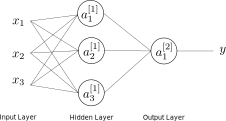
\includegraphics[width=0.75\textwidth]{Chapter3/neuralnet.pdf}
    \caption{Simple neural network.}
    \label{fig:neuralnet}
\end{figure}

Every node of the network is computed using the values from the previous layer. 
For the MLP, the node computation model is done through
a linear model $f(x; \theta)$, with $\theta$ consisting of internal parameters $w$ (weights) and $b$ (bias).
$w$ has the same dimensions as the input and $b$ is a scalar.
In this work, we treat $w$ as a column vector.

\begin{equation}
    w = \begin{bmatrix}
            w_1 & w_2 & w_3 & w_4 & \dots & w_{n-1} & w_{n}
        \end{bmatrix}^\intercal
\end{equation}

The model is defined as

\begin{equation}
    z = w^Tx + b
\end{equation}

The output of the node $a$, also known as the activation, is calculated with $x$, $b$ and 
a function $\sigma : \mathbb{R} \rightarrow \mathbb{R}$:

\begin{equation}
    a = \sigma(z) = \sigma(w^T x + b) = \sigma \bigg(\sum_{i=1}^n w_i x_i + b \bigg)
\end{equation}

Figure \ref{fig:neuralnet_out} illustrates the output of a single neuron.

\begin{figure}[ht]
    \centering
    \includegraphics[width=0.6\textwidth]{Chapter3/neuralnet_output.png}
    \caption{Node computation.}
    \label{fig:neuralnet_out}
\end{figure}

$\sigma$ is called activation function, applied to the model output ($z$).
The activation function normally is a non-linear function and its most used common choice
today is the \textbf{rectified linear unit} \cite{ReLU} or ReLU
and is defined as $\sigma(z) = max\{z, 0\}$, shown in \ref{fig:relu}. 

\begin{figure}[h]
    \centering
    \includegraphics[width=0.75\textwidth]{Chapter3/relu.pdf}
    \caption{Linear rectified unit plot.}
    \label{fig:relu}
\end{figure}

Other examples of popular activation functions are $\sigma(z) = \frac{1}{1 + e^{-z}}$, known as the sigmoid function
and $tanh(z)$ \cite{ActivationFunction}.

A neural network is therefore is a connection of multiple neurons as inputs to other neurons.
Let us return our attention to the network from Figure \ref{fig:neuralnet}.
We denote $(W,b) = (W^{[1]}, b^{[1]}, W^{[2]}, b^{[2]})$ as the network parameters, where $W^{[l]}$ is 
the matrix formed by concatenating the individual parameters of the $l$-th layer such that
$W_{ij}$ denotes the parameter associated with the connection between neuron $j$ from the $l$-th layer 
and neuron $i$ from layer $l + 1$.
Similarly, $b^{[l]}$ is the concatenation of the biases $b$ of each neuron of layer $l + 1$ and 
$b_i^{[l]}$ the bias of the $i$-th neuron of layer $l + 1$.

For the network depicted in Figure \ref{fig:neuralnet}, we are now capable of calculating the output $y$.

For the first layer: 

\begin{equation}
    z^{[1]}  = W^{[1]}x + b^{[1]} 
\end{equation}

\begin{equation}
   a^{[1]}  = \sigma(z^{[1]})
\end{equation}

And for the second layer:

\begin{equation}
    z^{[2]} = W^{[2]}a^{[1]} + b^{[2]}
\end{equation}

\begin{equation}
    y = a^{[2]} = \sigma(z^{[2]})
\end{equation}

We can think of the neural network as a recursive structure where each activation is calculated with the past's layers activation.
$a^{[l]}$ can be computed as:

\begin{equation}
    z^{[l]} = W^{[l]}a^{[l-1]} + b^{[l]}
    \label{eq:nn}
\end{equation}

\begin{equation}
    a^{[l]} = \sigma(z^{[l]})
\end{equation}

Note also that $a^{[1]} = x$.

\subsection{Vectorization}

In the previous section, we focused on computing the output of the neural network given a single sample $x$.
In modern days, however,  we are normally interested in calculating the output of a neural network for thousands or even millions of samples.

For $m$ samples, we could naively compute the output of the neural network for each example $x^{(i)}$ with Algorithm \ref{algo:naive_sample_algo}.

\begin{algorithm}[H]
    \DontPrintSemicolon
    \SetAlgoLined
    \KwResult{Output of NN for m samples.}
    \For{i = 1 to m}{
       $a^{[0]} = x^{(i)}$\;
        \For{j = 1 to L}{
            $z^{[j](i)} = W^{[j]}a^{[j-1](i)} + b^{[j]}$\;
            $a^{[j](i)} = \sigma(z^{[j](i)})$\;
        }
        $y^{(i)} = a^{[l](i)}$\;
    }
    \caption{Naive algorithm for computing NN output of $m$ samples.}
    \label{algo:naive_sample_algo}
\end{algorithm}

In practice this algorithm runs relatively slow since it computes the output of the network sequentially for each sample and 
we will apply vectorization to achieve a much faster algorithm.

Firstly, Vectorization is a technique that transforms a set of computations done sequentially in a for loop into matrix operations.
We will now vectorize our initial problem.

Let us define the following matrices

\begin{itemize}
    \item $X$ is a matrix where column i is the i-th sample $x^{(i)}$ and $W^{[l]}$. 
    We can analogously define matrices A and Z.
        $ X = \begin{bmatrix}
        x^{(1)} & x^{(2)} &  \dots  & x^{(m)} 
        \end{bmatrix}$.

    \item $W^{[l]}$ is the  weight matrix for the $l$-layer, as defined in Section \ref{sec:rep}. 
        % $ W^{[l]} = \begin{bmatrix}
        % \left(w^{[1]})\right)^T \\ \left(w^{[2]})\right)^T \\  \vdots  \\\left(w^{[l]})\right)^T} 
        % \end{bmatrix}$.
    \item $b^{[l]}$ is the bias vector for layer $l$, as defined in Section \ref{sec:rep}.
        % $ B^{[l]} = \begin{bmatrix}
        % b^{[1]} \\ b^{[2]} \\  \vdots \\ b^{[l]}
        % \end{bmatrix}$.
\end{itemize}

For the vectorized version of Algorithm \ref{algo:vectorized_sample}.

\begin{algorithm}[H]
    \DontPrintSemicolon
    \SetAlgoLined
    \KwResult{Output of NN for m samples.}
    \For{j = 1 to L}{
        $Z^{[j]} = W^{[j]}A^{[j-1]} + b^{[j]}$\;
        $A^{[j]} = \sigma(Z^{[j]})$\;
    }
    \caption{Vectorized algorithm for computing NN output of $m$ samples.}
    \label{algo:vectorized_sample}
\end{algorithm}

The vectorized version is much better since these matrices operations can be greatly sped up
on GPUs or hardware that have support for Streaming SIMD Extensions (SSE). The great majority of 
popular deep learning libraries use as much vectorization as they can.

\subsection{Deep Neural Networks}

We can extend the architecture we saw on Section \ref{sec:rep} to a higher number of layers called
deep neural networks. Figure \ref{fig:deepnn} illustrates a neural network with multiple hidden layers.

\begin{figure}[h]
    \centering
    \includegraphics[width=1\textwidth]{Chapter3/deep_neural_net.png}
    \caption{Neural network with multiple layer.}
    \label{fig:deepnn}
\end{figure}

The activation of layer $l + 1, l > 1$, can be calculated according to Equation \ref{eq:nn}.

\section{Learning}

As described in the previous section, feedforward networks defines a mapping $y = f(x; \theta)$,
or, equivalently, serve as general function approximators.

This section describes deep learning algorithms that learn the value of the parameters $\theta$ that best approximates $f$.

Most deep learning algorithms need to describe a cost function and optimization algorithm.

\subsection{Cost Function}

The cost function $J(\theta)$ is a metric of how good our estimator is to our dataset: the lower the cost function, the less error
the model has when predicting $y$. It describes the function that we wish to minimize and normally it envolves an average of the errors
between the the target value of a sample and the predicted value of the estimator for the sample.

For example, for the problem of linear regression where $X$ are the sample values and $y$ are the target
values for our dataset, we wish to learn the parameters $\theta$ from our function approximator $f$. 
The most used cost function for this problem is

\begin{equation}
    J(\theta) = \dfrac{1}{m} \sum_{i = 1}^m (y_i - f(x_i, \theta))^2
\end{equation}

Another example is the logistic regression problem. The most common cost function for this problem is

\begin{equation}
    J(\theta) = - \dfrac{1}{m} \sum_{i = 1}^m [y_i\log{f(x_i, \theta} + (1 - y_i)\log{1 - f(x_i, \theta)}]
\end{equation}

Choosing a good cost function greatly impacts how good the design of the deep neural network is.

% TODO Regularization

\subsection{Optimization Algorithms}

After defining a cost function, finding the parameters that effectively minimize the cost function is not trivial.
The non linearity of NN causes most cost functions to be non-convex and therefore, neural networks are usually
trained by iterative, gradient-based optimizers. In practice, however, this is very unlikely
 \cite{swirszcz2017local, goodfellow2014qualitatively, lin2017does}.

Section \ref{subsec:back_prop} describes how neural networks gradients can be calculated.

\subsubsection{Gradient Descent}

One of the most common optimization algorithm is Gradient Descent. It is an iterative first-order method
that tries to find a local minimum for a function $f$ by moving in the negative direction of its gradient.
Specifically for neural networks, our goal is to minimize the cost function $J(\theta)$. The algorithm's update step
is Equation \eqref{eq:grad_desc} done for each $\theta_i$

\begin{equation}
    \theta_i = \theta_i - \alpha \dfrac{\partial J}{\partial \theta_i}
    \label{eq:grad_desc}
\end{equation}

The learning rate, $\alpha$ measures how big the update step in the direction of the gradient will be.

For example, let $g:\mathbb{R}^2\to\mathbb{R}$ given by $g(x,y)=y \sin(x) - x\cos(y)$. Figure \ref{fig:grad_desc}
illustrates 5 steps of the gradient descent algorithm. Notice how the red circle is the starting point and after 
the last iteration, the algorithm arrives approximately at a local minimum.

\begin{figure}[ht]
    \centering
    \includegraphics[width=0.8\textwidth]{Chapter3/func_exam.pdf}
    \caption{Gradient descent on function g.}
    \label{fig:grad_desc}
\end{figure}

\subsubsection{Stochastic Gradient Descent}

Another popular algorithm is Stochastic Gradient Descent (SGD) that is a stochastic approximation of Gradient Descent.
Instead of calculating $J(\theta)$ as an average between all the samples, the gradient update step is done once per sample.
It calculates an approximation of the gradient and updates the parameters $\theta_i$ with every sample.
Algorithm \ref{algo:sgd} describes SGD

\begin{algorithm}[H]
    \DontPrintSemicolon
    \SetAlgoLined
    \KwResult{Function minimum}
    \While{An approximate minimum is not obtained} {
        Randomly shuffle examples in the training set\;
        \For{i = 1,2,..., m} {
            $\theta_i = \theta_i - \alpha \nabla J_i(\theta)$\;
        }
    }
    \caption{SGD algorithm.}
    \label{algo:sgd}
\end{algorithm}

The gradient approximation for SGD is much faster to compute, however, since it is a noisy estimate of the gradient,
SGD may need more steps to converge to a local minimum.

\subsubsection{Mini-Batch Gradient Descent}
Finally, Mini-Batch Gradient Descent combines the idea from Gradient Descent and SGD.
It computes the gradient using more than one training example, called a \textit{mini-batch}, at each step. It may result
in smoother convergence and the code can be accelerated by making use of vectorization.

\section{Back Propagation}
\label{subsec:back_prop}

We have seen how a few gradient-based optimization algorithms work. 
To minimize the cost function we need to compute the partial derivatives of the cost function w.r.t. 
to each weight of the neural network. Calculating these partial derivatives manually would be computacionally
infeasible for large networks.
In deep neural networks, by using the chain rule, we can calculate the partial derivatives in an efficient and
compact way.

Backpropagation is an algorithm that computes the gradients of the loss function w.r.t. each input from the network.

% % Gradient image

% Therefore numerical gradient computation is an important step in deep learning.


\chapter{Deep Reinforcement Learning}
\label{chap:deep_rl}
The previous two chapters described the background for RL and DL. In this chapter, we will see 
how these two fields are combined in powerful state-of-the-art algorithms for solving complex reinforcement learning problems.
In this work, we use all the algorithms presented in this chapter.

\section{Deep Deterministic Policy Gradients (DDPG)}

DDPG \cite{DDPG} is an off-policy actor-critic algorithm that simultaneously estimates the policy and the action-value function.
It has two major components (denoted by the actor and the critic):

\begin{itemize}
    \item Actor function $\mu(s \vert \theta^\mu) $ that represents the current policy, mapping states to specific actions.
     It is a policy function approximator using deep neural networks.
    \item Critic function $ Q(s, a \vert \theta^Q)$ that approximates the Q function. 
    It is value function approximator using deep neural networks.
\end{itemize}

DDPG is an extension of the Deterministic Policy Gradient Algorithm (DPG) \cite{DPG}. 
DPG introduces a very important theorem for policy gradient methods that extends the standard policy gradient
theorem for stochastic policies to deterministic policies.

The theorem states: 

% Explain the theorem better

\begin{equation}
\begin{split}
    \nabla_{\theta^\mu} \mu
        & \approx \mathbb{E}_{s_t \sim \mu'}
                [\nabla_{\theta^\mu} Q(s, a \vert \theta^Q)\vert_{s=S_t,a=\mu(S_t \vert \theta^\mu)}]  \\
        & = \mathbb{E}_{s_t \sim \mu'}
                [\nabla_a Q(s, a \vert \theta^Q)\vert_{s=S_t,a=\mu(S_t)}
                \nabla_{\theta_\mu}\mu(s\vert\theta^\mu)\vert_{s=S_t}]
\end{split}
\label{eq:dpg}
\end{equation}

Equation (\ref{eq:dpg}) proves that a deterministic policy gradient can be estimated by the estimated
action-value function's gradient.
DDPG's policy update is based on Equation (\ref{eq:dpg}) and adapts some key ideas from Deep Q-Networks (DQN) \cite{RLNature2015}:
DQN introduces 2 modifications to standard Q-learning algorithm to make it suitable for training
large neural networks without diverging.

\begin{itemize}
    \item Use of a technique known as experience replay. It consists of storing the agent's experiences at each timestep in a 
    dataset so that during the Q-learning updates (inner loop of Algorithm \ref{algo:ddpg}) we use samples of experiences.
    This approach allows for greater data efficiency and the randomization breaks the correlations between temporal data.
    \item Use a copy of the actor and critic as target networks. The target network is updated at a lower frequency
    using the weights of the network $Q$. This improves stability compared to standard Q-learning.
\end{itemize}

DDPG is based on Equation (\ref{eq:dpg}) and uses these ideas from \cite{RLNature2015} applied to the continuous domain.
A major challenge, however, of learning in continuous action spaces is exploration. DDPG and other off-policy algorithms
can explore independently from learning. DDPG employs an exploration policy $\mu'$ by adding noise sampled from a noise process
$\mathcal{N}$ to the actor policy according to:

\begin{equation}
    \mu'(S_t) = \mu(S_t \vert \theta^\mu) + \mathcal{N}
\end{equation}

A novel approach that tackles the problem of action exploration is adding noise to the parameter space,
instead of on the action space \cite{OpenAIParameterNoise}. This is done by adding adaptive noise to
the parameters of the neural network policy and this helps algorithms better explore their environments.
We use this type of exploration in this work.
Figure \ref{fig:parameter_noise} illustrates the differences between action space and parameter space noise.

\begin{figure}[thb]
    \centering
    \includegraphics[width=0.6\textwidth]{Chapter4/parameter_noise.png}
    \caption{Comparison between action space noise (left) and parameter space noise (right).
    Extracted from \cite{OpenAIParameterNoise}.}
    \label{fig:parameter_noise}
\end{figure}

Algorithm \ref{algo:ddpg} describes DDPG.

\begin{algorithm}[H]
    \DontPrintSemicolon
    \SetAlgoLined
    % \KwResult{Trained policy \theta^{\mu}}
    Randomly initialize critic network $Q(s, a \vert \theta^Q)$ and actor $\mu(s \vert \theta^\mu)$ 
    with weights $\theta^Q$ and $\theta^\mu$. \;
    Initialize target network $Q'$ and $\mu'$ with weights $\theta^{Q'} \leftarrow \theta^Q$, $\theta^{\mu'} \leftarrow \theta^\mu$.\;
    Initialize replay buffer $R$. \;
    \For{episode = $1$, $M$}{
        Initiliaze a random process $\mathcal{N}$ for action exploration. \;
        Receive initial observation state $S_t$. \;
        \For{t = $1$, $T$}{
            Select action $A_t = \mu(S_t \vert \theta^\mu) + \mathcal{N}_t$ according to the current policy and exploration noise.\;
            Execute action $A_t$ and observe reward $R_t$ and observe new state $S_{t+1}$.\;
            Store transition $(S_t, A_t, R_t, S_{t+1})$ in $R$. \;
            Sample a random minibatch of $N$ transitions $(S_i, A_i, R_i, S_{i+1})$. \;
            Set $y_i = r_i + \gamma Q'(S_{i + 1} , \mu'(S_{i + 1} \vert \theta^{\mu'}) \vert \theta^{Q'})$. \;
            Update critic by minimizing the loss: $L = \dfrac{1}{N} \Sigma_i(y_i - Q(S_i, A_i \vert \theta^Q))^2$. \;
            Update the actor policy using the sample policy gradient: \;
            \Indp\Indp
                $ \nabla_{\theta^\mu}J \approx  \dfrac{1}{N} \nabla_a Q(s, a \vert \theta^Q)\vert_{s=S_t,a=\mu(S_t)}
                \nabla_{\theta_\mu}\mu(s\vert\theta^\mu)\vert_{s=S^t}]$ \;
            \Indm\Indm
            Update the target networks: \;
            
            \Indp\Indp
                $\theta^{Q'} \leftarrow \tau \theta^Q + (1 - \tau)\theta^{Q'}$ \;
                $\theta^{\mu'} \leftarrow \tau \theta^\mu + (1 - \tau)\theta^{\mu'}$ \;
                \;
        }
    }
    \caption{DDPG algorithm}
    \label{algo:ddpg}
\end{algorithm}

The main issue of DDPG is that the step size for the gradient update is a hyperparameter that has to be chosen
and must fall into the right range to achieve good performance.
There is no guarantees that the policy will improve and the following algorithms address this issue.

\section{Trust Region Policy Optimization}

Trust Region Policy Optimization (TRPO) is an iterative procedure for optimizing policies \cite{TRPO}. The algorithm alternates between
sampling data by interacting with the environment and optimizing an alternate (``surrogate") objective function subject to a 
constraint on the size of the policy update that guarantee monotonic improvement.
Similarly to DDPG, the policy is also represented as a fully-connected neural network.

TRPO is an on-policy algorithm that improves upon REINFORCE \cite{REINFORCE} by computing an ascent direction that ensures a small change in the policy distribution.
This algorithm uses the Kullback–Leibler (KL) divergence to constrain the policy step size to lie within a (trust) region.
The KL divergence is a measure of how one probability distribution diverges from a second 
and it is defined as the relative entropy between two continuous random variables $P$, $Q$ (and similarly for discrete probability distributions).
Let $p(x)$ and $q(x)$ be the probability density function of $P$ and $Q$ respectively, the KL divergence, $KL[P, Q]$, is defined by:
\begin{equation*}
    KL[P, Q] = \int_{- \infty}^{+\infty} p(x) log \dfrac{p(x)}{q(x)}dx
    \label{eq:kl}
\end{equation*}

TRPO tries to solve the following second-order constrained optimization problem:

\begin{flalign}
    &\underset{\theta}{\text{maximize  }} \hat{\mathbb{E}}_t\Bigg[\dfrac{\pi_{\theta}(a_t \vert s_t)}{\pi_{\theta_{\text{old}}} (a_t \vert s_t) } \hat{A}_t \Bigg] \\
    & \text{subject to  } \hat{\mathbb{E}}_t[KL[\pi_{\theta_{\text{old}}}(\cdot \vert s_t), \pi_{\theta}(\cdot \vert s_t)]] \leq \delta
\end{flalign}

Here $\hat{\mathbb{E}}_t[. . .]$ is the empirical average over a finite batch of samples and $\hat{A}_t$ is an estimator for the advantage function
at timestep $t$. 
The advantage function $A(A_t, S_t) = Q(A_t, S_t) - V(S_t)$ 
is an estimate of how good taking a specific action in a given state is compared to the average of all possible actions.
TRPO uses the conjugate gradient algorithm to solve this constrained optimization.

The policy, denoted as the conditional probability distribution $\pi_\theta (a \vert s)$ is parameterized with a 
neural network.
The neural network deterministically maps the state vector $s$ (the input) to a vector $\mu$, which parameterizes the distribution.
The action $a$ is then sampled from this parameterized distribution.

For our experiments in this work with continuos state and action spaces, we define the policy by a normal distribution
$\mathcal{N}$ where the mean and log standard deviation are outputs of a neural network \cite{TRPO}.

One of the novel ideas introduced by TRPO is limiting the step size of the policy (using the KL divergence) to guarantee policy improvement. 
However, despite being data efficient and reliable in comparison to DDPG, TRPO is computationally very expensive
 and its implementation is relatively complicated \cite{PPO}.

\section{Proximal Policy Optimization (PPO)}

PPO is very similar to TRPO but tries to optimize a different surrogate objective function \cite{PPO} with the purpose of being simpler and
computationally less intensive than its counterpart. PPO uses only first-order optimization

Let $r_t(\theta) = \dfrac{\pi_{\theta}(a_t \vert s_t)}{\pi_{\theta_{old}}(a_t \vert s_t)}$. Note that when there is no update to the policy,
$r_t({\theta_{\text{old}}}) = 1$.

The main surrogate objective for PPO is

\begin{equation}
    L(\theta) = \hat{E}_t\big[\text{min}(r_t(\theta)\hat{A}_t, \text{clip}(r_t(\theta), 1 - \epsilon, 1 + \epsilon)\hat{A}_t\big]
\end{equation}

$\text{clip}$ is a function $f : \mathbb{R} \rightarrow \mathbb{R}$ defined as

\begin{align*}
    clip(x) = \begin{cases}
        -1, & \mbox{if } x < -1 \\
        x, & \mbox{if } -1 \leq x \leq 1 \\
        1, & \mbox{if } x < 1
        \end{cases}
\end{align*}

$L(\theta)$ is the loss function and  $\hat{A}_t$ is an estimator for the advantage function
at timestep $t$. This objective can further be improved by adding an entropy bonus to incentivize exploration \cite{REINFORCE, A3C}.

Similarly to the TRPO algorithm,
the policy is represented as a fully-connected MLP that outputs the mean of a gaussian distribution and
the action $a$ at each timestep is sampled from this distribution.

This algorithm is far less intensive to optimize and also removes the KL divergence constraint resulting in a
first order optimization problem.
Also, empirically, it has a better performance than TRPO, and allows parallel implementations and is very data efficient.

\chapter{Methodology}
\label{chap:method}
This chapter focuses on describing the set of tools used for this work.

% EXPLAIN  MORE ABOUT THIS CHAPTER


\section{Tools}

This section describes the tools that made this work possible.

\subsection{C++}

C++ is a general purpose programming language that is highly efficient and flexible.
It is greatly focused on performance allowing low-level memory manipulation \cite{C++}.

The ITAndroids Soccer3D base code was already in C++ and therefore, anything that interacts with the soccer simulation server
was also in C++ to integrate seamlessly with the codebase.
For this work, we used version 14 which is the most recent standardized (and stable) version.

\subsection{Python}

Python is an interpreted general purpose high-level programming language \cite{Python}. It has an easy-to-read syntax
closely resembling pseudocode therefore it allows faster development time which makes it easy to prototype new ideas.
For these reasons, the scientific community's usage of Python has greatly increased in recent years, even more so in the
deep learning community. 

For this work, we chose version 3.5 since it is the most recent and stable version when starting development.


\subsection{Protocol Buffers}

Protocol Buffers is a multiplatform library for serializing structured data that supports multiple programming languages \cite{ProtoBuf}.
It is very useful for developing uncoupled client-server applications that communicate using a simple and flexible API.

For these reasons, we chose Protocol Buffer as the client-server API.

\subsection{OpenAI Gym}

OpenAI Gym is a toolkit for running reinforcement learning algorithms in different environments \cite{OpenAIGym}.
It allows testing and benchmarking RL algorithms by providing a standardized set of environments.
This is very important for RL since it makes it accessible for the research community to compare different algorithms \cite{OpenAIGymPaper}.

Figure \ref{fig:openai_env} illustrates a few example environments from OpenAI Gym.

\begin{figure}[H]
    \centering
    \includegraphics[width=1\textwidth]{Chapter5/openai_env.png}
    \caption{OpenAI Gym environments, extracted from \cite{OpenAIGym}.}
    \label{fig:openai_env}
\end{figure}

Because of these reasons, OpenAI Gym was used in this work.

\subsection{TensorFlow}

TensorFlow is an open source software library for numerical computation using data flow graph \cite{TensorFlow}.
It is greatly used for machine learning applications since it provides efficient implementation of gradient computations and
optimization algorithms that can be parallelized by making use of specialized hardware instructions like SSE and GPU.
The library also exposes an API for multiple languages such as Python, C++, Go and Java.

TensorFlow was chosen because of its big developer community and its various tools available such as Tensorboard, a
visualization dashboard that is very useful for debugging and plotting.

\section{Simulation Environment}

The chosen simulation environment is the \textit{SimSpark} simulator \cite{SimSpark}. 
It is a simulation system for multi-agent simulations and uses Open Dynamics Engine \cite{ODE} for rigid body dynamics and collision detecting.
The system allows two teams of up to eleven humanoid robots to play against each other.

The implementation of SimSpark does not guarantee that events are reproducible and adds noise to the problem.
This makes the problem more challenging to learn, since different instances of the same simulation may have different outcomes.
In addition, it is very important to run the RL algorithms multiple times to reduce the variance in the outcomes.

The server also exposes a network interface that allows external processes to be notified of the simulation's state
for purpose of visualization or logging. This interface allows queries of the ground truth state of 
the simulation state that are not available during regular game play, e.g. the global position of the robot.
The entity that reveals the ground truth is known as the Wizard in the ITAndroids code.

For this work, we used \textit{RoboViz}, a publicly available visualization tool created by Justin Stoecker \cite{RoboViz} that allows a few
improvements over the default visualization tool. Figure \ref{fig:sim3d} shows a typical game scene between two teams inside \textit{RoboViz}.

\begin{figure}[H]
     \centering
     \includegraphics[width=0.95\textwidth]{Chapter5/sim3d.png}
     \caption{\textit{SimSpark} Simulation Environment running.}
     \label{fig:sim3d}
\end{figure}

Agents communicate with the simulator via TCP connections. The agent communicates with the server and the server
executes a simulation step of $\Delta t = 0.020$ s. At each timestep, the robot sends the desired speed values of each joint to the server
and this is how the agents perform actions within the simulation \cite{SimSparkEffectors}.

Our simulated agent is a simulation of the Nao humanoid robot manufactured by SoftBank Robotics \cite{NaoRobot} and has 22 joints (or degrees of freedom).
Therefore, to make the robot act as desired, at each timestep, we must calculate all 22 joint velocities for the robot.
Figure \ref{fig:nao} depicts the real Nao robot.

\begin{figure}[H]
    \centering
    \includegraphics[width=0.25\textwidth]{Chapter5/nao.png}
    \caption{SoftBank Robotics Nao.}
    \label{fig:nao}
\end{figure}

The main reason this simulation environment was chosen was that it is the official simulator used in RoboCup Soccer Simulation 3D competition since 2004.

\section{Walking Engine}

The omnidirectional walking engine is an algorithm that calculates how the humanoid robot should walk. 
As input, it receives a desired velocity $v = [v_x, x_y, x_{\psi}]^T$ , where $v_x$, $v_y$ and $v_{\psi}$
are speeds in the forward, lateral and rotational directions, respectively and calculates the robot's joint angles as output.
These angles are then fed to PID controllers at each joint to compute the joint velocities actually sent to the server.
A simplified overview of the walking engine is shown in Figure \ref{fig:walkingengine}.
In this work, we are not interested in the walking engine per se, however it is important to understand some low-level aspects
of the walking engine since it implies in some design restrictions on how the robot walks and influences the learned behavior.

A popular concept in the humanoid literature is the Zero Moment Point (ZMP) \cite{ZMP}.
The ZMP can be thought of the dynamic version of the center of mass (CoM) due to the following stability
criterion: a biped is dynamically stable at a given time instant if the ZMP is inside the support polygon
(the convex hull of all contact points on the ground) \cite{ZMP}.
The walking engine we use is based on \cite{MestradoManga, CaminhadaManga}.
The engine is based on the Zero Moment Point (ZMP)
and approximates the robot dynamics using the Linear Inverted Pendulum Model \cite{Kajita}.

The walking engine can be described as the following components:

\begin{itemize}
    \item \textbf{Footstep planner:} decides the torso and swing foot poses of the robot at the end of the step.
    \item \textbf{CoM Trajectory Generator:} determines the trajectory for the CoM in order to achieve these planned poses.
    Essentially, the ZMP must always be within the support polygon during a step and the CoM trajectory must always
    match the CoM positions at the beginning and at the end of the step. This defines a boundary value problem that can
    be solved analytically and the solution describes the trajectory for the CoM.
    \item \textbf{Swing Foot trajectory Generator:} determines the trajectory for the swing foot by interpolating between
    the initial and final poses of the robot's feet. 
    \item \textbf{Inverse Kinematics (IK) Solver:} calculates the joint angles through IK.
\end{itemize}

A simplified overview of the walking engine is shown in Figure \ref{fig:walkingengine}.

\begin{figure}[htb]
    \centering
    \includegraphics[width=0.95\textwidth]{Chapter5/walkingengine.png}
    \caption{Walking Engine overview.}
    \label{fig:walkingengine}
\end{figure}

The walk cycle, shown in Figure \ref{fig:walk_cycle} has constant duration $T$ and the support foot always alternates between
the right and left, having two double support phases in each step.

\begin{figure}[ht]
    \centering
    \includegraphics[width=0.7\textwidth]{Chapter5/humanoid_step.png}
    \caption{Walk cycle (a step).}
    \label{fig:walk_cycle}
\end{figure}

Also, for stability purposes, the acceleration is bounded, so it may take multiple walking steps to 
reach the desired speed. For details, please  refer to \citen{MestradoManga}.

\section{Metrics}
\label{sec:metrics}

When trying to solve some reinforcement learning task, it is very important to define a few metrics
that effectively provides information during the training stage. With this information we try to understand
how well the agent is doing in its task.
In this work, we focused on 2 main metrics:

\begin{itemize}
    \item \textbf{Episode accumulated reward:} Maximizing the episode return is the goal of RL therefore
     it is the most obvious performance indicator and gives a very good sense of how well the agent's actions are doing.
    \item \textbf{Episode duration:} Episode reward is the central element in the RL framework to describe how
    well the agent is doing, however, for some further intuition, 
    it is also interesting to observe how long each episodes is taking in time.
    For example, for the \textit{Racing Domain}, if the episode is finishing early, it is a good indicator
    that the robot is falling or leaving the race track early.
    \item \textbf{Data efficiency:} A quantitative measure of how long an agent takes to learn a good behavior.
\end{itemize}

These are the metrics we used for all the tasks however. 
We have also made use of task specific metrics that further try to measure the agent's performance.
These metrics are described in Chapter \ref{chap:contrib}.

All the metrics were calculated in an offline manner, that is, after the simulation finished.
This was possible since we logged all the state and action information from the agent for each episode on the server side
and was very helpful for reviewing past runs to extract non-obvious conclusions from the data.

\chapter{Learning Kick Behaviors}
\label{chap:contributions}

The major contribution of this work is providing a task modeling and setup for learning humanoid  movements in the RoboCup Soccer3D domain using reinforcement learning frameworks. More specifically, we learned several variations of a kick motion, creating behaviors capable of imitating the ZMP kick, reaching a much farther position for the ball, and reaching a desired fixed final distance for the ball.


We also introduce the deep mimic approach for this class of problems and a specific curriculum to learn, as well as several implementation considerations, manually tunned and developed after a few iterations.

\section{Environment and Implementation}

As previously mentioned in Chapter \ref{chap:method}, this work used the RL algorithms implementations from the OpenAI baselines repository \cite{baselines}. More specifically, the high-quality implementation of PPO. Not implementing the DRL algorithms from scratch made it much easier to test, iterate, improve and focus on developing the agent experiments.

The PPO implementation on Baselines was adapted to change the communication with the OpenAI Gym environments to communicate with the Soccer3D agent, maintaining the same function protocols.

The framework used to integrate the baselines code with new experiments, flexible to develop, in the Soccer3D domain was already built in the work \cite{TGMuzio}. This framework can be basically described by its two main modules, each one running as a separate process and communicating through Protocol Buffers.

\begin{itemize}
\item \textbf{Learning Client:} Process that runs the reinforcement learning algorithms and makes remote procedure calls (RPCs) to the server, exchanging state/action information with the soccer agent. This module was implemented in Python 3.5 and TensorFlow, using OpenAI Baselines implementations.

\item \textbf{Soccer Agent:} The simulated agent which interacts with \textit{SimSpark} and with the learning client, executing the learning experiments. This module was implemented in C++ and uses the ITAndroids Soccer Simulation 3D code base.
\end{itemize}

As already commented, the API between server and client uses Protocol Buffers, with the exchange of RPCs containing the standard state, action, reward and end of episode information used in OpenAI Gym. An illustration of this framework follows in the diagram presented in Figure \ref{fig:RL_framework}. For details, please refer to \cite{TGMuzio}.

\begin{figure}[H]
    \centering
    \includegraphics[width=0.8\textwidth]{Chapter6/architecture.png} 
    \caption{Learning Architecture diagram. Extracted from \cite{TGMuzio}}
    \label{fig:RL_framework}
\end{figure}

\section{Infrastructure}

This work used the Intel AI DevCloud as its main infrastructure to run all learning experiments described below.

The cluster is composed by 10 computation nodes using each one a 24 cores Intel Xeon processor. Furthermore, the experiments setup exploited the parallelization feature of PPO, running up to 12 Soccer Agents per node, besides the Learning Client process, and collecting a total number of samples in the magnitude of 100 million.

\section{Deep Mimic Learning}
\label{sec:deep_mimic}

The Deep Mimic approach \cite{deepmimic} established a great new paradigm in which this work was based on. It introduces a novel idea of allowing the supply of reference motions from motion capture or hand-authored animation data for style, and then generating goal-directed and physically realistic behavior from those reference motions \cite{deepmimic}.

The basic approach presented for this mission consists in rewarding the agent to reproduce motions that resemble the reference data, as well as to achieve additional task objectives.

A control policy $\pi (a_t|s_t,g_t)$ maps the state of the character $s_t$ and a task-specific goal $g_t$ to an action $a_t$. The action distribution is gaussian, with fixed covariance and mean given by a neural network. This policy outputs the desired joints positions, which is later translated into torque commands by each joint PD controller.

The overall reward is splitted into the imitation reward, given by $r_I(s_t,a_t)$, and the task-specific reward, given by $r_G(s_t,a_t)$. The final reward is therefore given by Equation \eqref{eq:deep_mimic_reward}.

\begin{equation}
r_t = \omega^I r_t^I + \omega^G r_t^G
\label{eq:deep_mimic_reward}
\end{equation}

The policies are trained with PPO using the clipped surrogate objective, maintaining also a further network for the value function $V_{\psi}(s,g)$.

It is worth mentioning that this work introduces also two novel ideas which significantly increased the robustness and performance of the learning behaviors. 

\begin{itemize}
\item \textit{Reference State Initialization} (RSI) randomly selects a state in which the agent and its reference actor begins at each episode. In this way, it makes possible to discover high reward future states without the need to learn everything until then, which can be very significant in difficult tasks like backflips.

\item \textit{Early Termination} (ET) finishes the episode when the agent reaches any fruitless condition, such as a fall or joints collision. This process discourage undesirable behaviors and the exploration of bad states, therefore increasing the learning efficiency.
\end{itemize}

\section{Experiments}

In this section, we describe the learning experiments conducted in this work. The ultimate goal is learning a complete behavior capable of kicking the ball towards a planned final distance fed into the input of the policy, however, we started by learning simpler problems. These problems were very useful not only in providing a curriculum learning approach \cite{BengioCurrLearning} and therefore the basements to achieve the final goal, but also helping to validate all the setup, algorithms and to get a better understanding of the problem and the simulation environment limitations.

\subsection{Supervised Kick Learning}

The first tentative of learning a kick behavior was basically learning to imitate the reference kick movement using supervised learning techniques. Therefore, for this experiment, there was no need to use the RL setup or to run a learning agent.

Once the reference movement is deterministic, the neural network used has only one input given by time itself. Two fully-connected hidden layers follow, composed by 512 leaky-relu hidden units each one. Finally, we have a output layer given by 22 linear units, providing position commands for all 22 agent joints.

%For training, we used Adam optimization, applying 5 consecutive optimization cycles with 5000 epochs each one and decreasing the learning rate linearly, applying $10e^{-4}$, $8e^{-4}$, $6e^{-4}$, $4e^{-4}$, $2e^{-4}$ respectively for each cycle.

\subsection{Pure Mimic Learning}

The second checkpoint to achieve was still learning to imitate the reference movement, reaching the best possible precision. However, since we wanted also to validate and test the learning setup, we chose the reinforcement learning approach, using the Proximal Policy Optimization algorithm.

\textbf{State space:} Since the reference movement is deterministic and the commanded actions only depend of the point in time, the 1D observation space consists on the episode timestep solely, given by a multiple of the simulator unit step $0.02s$.

\textbf{Action space:} We decided to restrict the action space to the joints with biggest impact in the kick distance, in order to reduce the learning cost for this task. Therefore, the 6D action space consists on the position commands for the 6 joints of the kicking leg. These position commands are sequentially fed into PID controllers on each joint, in order to generate velocity commands to the motors, which are finally sent to Simspark. It is also worth mention that the other 16 joints will be driven by the ZMP kick engine.

\textbf{Reward signal:} The reward is given by:

\begin{equation}
r_t = -\sum_{j=1}^{6}{|q_t^j-\hat{q}_t^j|^2}
\end{equation}

Where $q_t^j$ and $\hat{q}_t^j$ represent the commanded positions to the j$th$ joint at instant $t$ from the learning agent and from the reference movement, respectively. Therefore, we basically penalize the square difference of the commands given to all 6 joints.

The reference movement used was the ZMP kick, described in the previous chapter. We also used a fully-connected NN with two hidden layers, and 512 leaky-relu units each one, followed by an output layer with 6 units.

Besides, in order to simplify the problem in a first moment, we ran everything offline, by comparing the network output with the reference data in a file, without the need to initialize the simulated agent. In this way, we can avoid the physical restrictions involved, and some limitations such as the robot falls, and therefore speeding up the learning process.

Furthermore, the biggest achievement from this task was obtaining a policy network that can also be used as the starting point for the following learning tasks. In this way, it already provides a big learning step in the process of reaching the ultimate goal.

\subsection{Farthest Final Distance Learning}
\label{sec:far_kick_description}

The following learning task consists in kicking the ball towards the longest possible distance. The purpose is testing the limits of the kick motion, and the deviation the learning process can achieve from the base movement.

We initialized the policy and value-function networks using the resulted ones from the pure mimic task. In this way, the agent already starts knowing a basic behavior for kicking. Therefore, the state and action spaces for this task is the same of the previous task, only requiring a special design for the reward signal.

The reward function was based on the Deep Mimic work \cite{deepmimic}, thus it follows the same format described in \eqref{eq:deep_mimic_reward}. The imitation component will then be given by Equation \eqref{eq:imitation_reward}, while the goal reward is described by Equation \eqref{eq:goal_reward_farthest}.

\begin{equation}
r^I_t = \omega^p r^p_t + \omega^e r^e_t + \omega^c r^c_t
\label{eq:imitation_reward}
\end{equation}

The imitation component in \eqref{eq:imitation_reward} is still composed by three other factors.

The pose reward $r^p_t$ is given by Equation \eqref{eq:position_imitation}, where $q_t^j$ and $\hat{q}_t^j$ represent the actual positions during motion of the j$th$ joint at instant $t$ from the learning agent and from the reference movement, respectively, and encourages the agent to match the joint orientations of the reference motion at each step.

\begin{equation}
r^p_t = exp \left[ -2 \left( \sum_{j=1}^{6}{|q_t^j-\hat{q}_t^j|^2} \right) \right]
\label{eq:position_imitation}
\end{equation}

The end-effector reward $r_t^e$ is given by Equation \eqref{eq:end_effector_imitation}, where $p_t^e$ and $\hat{p}_t^e$ represent the kicking feet positions from the learning agent and reference movement, respectively, and encourages the agent feet to match the positions from the reference movement.

\begin{equation}
r^e_t = exp \left[ -40 |p_t^e-\hat{p}_t^e|^2 \right]
\label{eq:end_effector_imitation}
\end{equation}

At last for imitation, the center-of-mass reward $r_t^c$ is given by Equation \eqref{eq:CM_imitation}, and penalizes the deviation between the agent CM $p_t^c$ and the reference CM $\hat{p}_t^c$.

\begin{equation}
r^c_t = exp \left[ -10 |p_t^c-\hat{p}_t^c|^2 \right]
\label{eq:CM_imitation}
\end{equation}

Finally, we have the goal reward component $r_t^G$ described in Equation \eqref{eq:goal_reward_farthest}. This expression basically encourages the longest distance between ball's final and initial positions, giving a big exponential reward. It is worth to notice that this reward signal is given at each episode timestep, encouraging also the agent to kick the ball as fast as possible.

\begin{equation}
r_t^G = exp \left[ 7 (\text{ballPos - ballInitPos}) \right]
\label{eq:goal_reward_farthest}
\end{equation}

This task was very useful in obtaining a new learned behavior for the first time, starting from the mimic base behavior. Hence, it helped to discover the limitations and particularities of this challenge, improving our overall knowledge about it.

\subsection{Fixed Final Distance Learning}

The next learning task consists in kicking the ball towards a fixed final distance, hardly inputed as a constraint in the reward function.

Following the same approach described for the Farthest Final Distance task in the previous section, in this task we also started with the policy and value-function MLPs developed in the Pure Mimic task. In this sense, we maintain the same state and action space.

The reward function follows the Deep Mimic design and is composed by a imitation component and a goal oriented component, described in \eqref{eq:deep_mimic_reward}. The imitation component has the same shape presented for the Farthest Final Distance task, introduced by Equations \eqref{eq:imitation_reward}, \eqref{eq:position_imitation}, \eqref{eq:end_effector_imitation} and \eqref{eq:CM_imitation}.

The goal reward component $r^G_t$, however, introduces a new design, specifically hard coded for each fixed distance experiment.

We conducted two experiments for learning to kick the ball towards the final positions of $0.8m$ and $1.5m$, however, it could be analogously replicated for other distances within the limits of the maximum distance reached in the previous task.

The goal reward function for the fixed positions of $0.8m$ and $1.5m$ experiments are given by Equations \eqref{eq:08_fixed_reward} and \eqref{eq:15_fixed_reward}, respectively.

\begin{equation}
10^4 exp \left( -10 |\text{ballFinalPos}-0.8| \right)
\label{eq:08_fixed_reward}
\end{equation}

\begin{equation}
10^4 exp \left( -10 |\text{ballFinalPos}-1.5| \right)
\label{eq:15_fixed_reward}
\end{equation}

The idea is to provide a big encouragement for reaching a final distance close to the desired target. This reward component is usually much bigger than the imitation one, in order to allow some significant deviations from the base movement capable of making possible to reach the goal.

Different than the Farthest Final Distance task, this goal reward component is only given at the end of the episode, after the ball stops, since we wanted to encourage precision rather than speed. This approach makes the reward function very sparse, introducing some challenges in the process.

The experiments implementation details, as well as the reward weights and hyperparameters will be presented in the next chapter.








\chapter{Experiments and Results}
\label{chap:experiments}


We conducted several experiments for each of the tasks described in Chapter \ref{chap:contributions}. Each experiment is composed of a training phase and a evaluation phase.

\begin{itemize}
\item Training phase: In this phase the agent is actually learning by sampling data from the simulation server to actively update the parameters of the policy and value-functions, represented as neural networks.

\item Evaluation phase: After the training phase, we freeze all the parameters and eliminate the exploration gaussian noise, turning the policy deterministic. Also, since we trained using RSI, for evaluation we initialize the state in a constant instant. Finally, we assess the training performance by the metrics described in section \ref{sec:metrics}.
\end{itemize}

We trained each task using the Proximal Policy Optimization (PPO) algorithm. After the learning phase is completed, we compare the final obtained movement with the classical ZMP kick, in order to evaluate the mimic performance in imitating the joints commands and also the goal performance in reaching the desired ball final position.

As described in section \ref{sec:devcloud}, the training phases for all experiments were conducted in the Intel AI DevCloud.

\section{Supervised Kick Learning}

In the Supervised Kick Learning task, we ran training using Adam optimization, applying 5 consecutive optimization cycles with 5000 epochs each one and decreasing the learning rate linearly, applying $0.001$, $0.0008$, $0.0006$, $0.0004$, $0.0002$ respectively for each cycle. The loss function used was the Mean Squared Error.

The other hyperparameters used follow the standard values found in the literature, also presented in table \ref{tab:SL}.

\begin{table}[ht]
    \begin{tabular}{|l|l|}
    \hline
    Hyperparameter            & Value    \\ \hline
    $\beta_1$ 	              & $0.9$ \\
    $\beta_2$                  & $0.999$     \\
    $\epsilon$                & $10^{-8}$     \\
    \hline
    \end{tabular}
\centering
\caption{Hyperparameters used Supervised Kick Learning.}
\label{tab:SL}
\end{table}

Figure \ref{fig:SL_MAE} shows the Mean Absolut Error for the first training cycle, and we can easily verify the efficiency for the training phase.

In the evaluation phase, we ran an agent using the obtained NN as the policy, and compared the joints commanded positions with the ZMP kick reference movement. Figure \ref{fig:SL_cmd_pos} shows the corresponding data for the right knee pitch joint.

\begin{figure}[H]
    \centering
    \includegraphics[width=0.6\textwidth]{Chapter7/plots/plot_MAE_supervised.pdf} 
    \caption{Mean Absolut Error - SL.}
    \label{fig:SL_MAE}
\end{figure}

\begin{figure}[H]
    \centering
    \includegraphics[width=0.6\textwidth]{Chapter7/plots/plot_joints_pos_superv.pdf} 
    \caption{Commanded Position for the Right Knee Pitch Joint - SL.}
    \label{fig:SL_cmd_pos}
\end{figure}

\section{Pure Mimic Learning}

In the Pure Mimic Learning experiment, we ran PPO with 1 simulated agent using  $2 \times 10^6$ total samples. The hyperparameters used are presented in table \ref{tab:ppo_pure_mimic}.

The key adaptations which made possible to learning this task were: increasing the NN size, since smaller networks showed to be unsuccessful in mapping all the movement details; and restricting the episode length to include only the phases with actual swinging foot, i.e, only the phases B, C and D of the ZMP kick described in section \ref{sec:ZMPkick}, which correspond to more subtle joints movements and with bigger influence in the ball's final position.

\begin{table}[ht]
    \begin{tabular}{|l|l|}
    \hline
    Hyperparameter            & Value    \\ \hline
    Adam stepsize             & $5 \times 10^{-5}$ \\
    Num. epochs               & $10$     \\
    Minibatch size            & $256$     \\
    GAE parameter ($\lambda$) & $0.95$   \\
    Discount ($\gamma$)		   & $0.99$	  \\
    Timesteps per batch       & $2048$   \\ \hline
    \end{tabular}
\centering
\caption{PPO hyperparameters used for Pure Mimic Learning.}
\label{tab:ppo_pure_mimic}
\end{table}

Figure \ref{fig:RL_mimic_reward} shows the total reward during the training phase, by its monotonic increasing we can see a clear success for this phase.

In the evaluation phase, we ran an agent using the obtained policy and compared joints positions commands. Figure \ref{fig:RL_cmd_pos} shows these commands for the Right Knee Pitch joint, comparing the mimic behavior with the ZMP kick reference movement. We can notice that that the NN commanded position contains a noise, corresponding to the gaussian exploration noise in the policy.

At the end, the agent was capable of kicking the ball towards the same final distance performed by the ZMP kick.

\begin{figure}[H]
    \centering
    \includegraphics[width=0.6\textwidth]{Chapter7/plots/plot_reward_mimic.pdf} 
    \caption{Reward signal during training for the mimic task.}
    \label{fig:RL_mimic_reward}
\end{figure}

\begin{figure}[H]
    \centering
    \includegraphics[width=0.6\textwidth]{Chapter7/plots/plot_joints_pos_mimic.pdf} 
    \caption{Commanded Position for the Right Knee Pitch Joint - mimic RL.}
    \label{fig:RL_cmd_pos}
\end{figure}

\section{Farthest Final Distance Learning}
\label{sec:far_kick_results}

In the Farthest Final Distance Learning experiment, we ran PPO with 20 simulated agents using $10^8$ total samples. The hyperparameters used are presented in table \ref{tab:ppo_far_kick}.

\begin{table}[ht]
    \begin{tabular}{|l|l|}
    \hline
    Hyperparameter            & Value    \\  \hline
    Adam stepsize             & $10^{-5}$ \\
    Num. epochs               & $10$     \\
    Minibatch size            & $2048$     \\
    GAE parameter ($\lambda$) & $0.95$   \\
    Discount ($\gamma$)       & $0.9999$ \\
    Timesteps per batch       & $4096$   \\ \hline
    \end{tabular}
\centering
\caption{PPO hyperparameters used for Farthest Final Distance Learning.}
\label{tab:ppo_far_kick}
\end{table}

The key adaptations which made possible to learn this task were: Performing the Random State initialization (RSI), described in the Deep Mimic Section \ref{sec:deep_mimic}; increasing the discount factor ($\gamma$); increasing the minibatch size; and performing very long trainings.

Since the greatest fraction of the goal reward is only received at the end of the episode, because the agent finishes the movement before the ball stops, the reward function is still quite sparse. Increasing the $\gamma$ and performing the random state initialization helped to deal with this limitation, making possible to propagate the reward signal into more initial states.

Increasing the minibatch size was useful to deal with the big noise in ball's terminal positions during training. Small variations given by the exploration noise in the joints' commands can result in big differences observed for the ball position. Increasing the batch size and running for multiple agents made possible to reach a more reliable gradient estimate.

Performing long trainings was essential, since the agent takes some time to actually starting to learn, as can be seen in the reward signal in Figure \ref{fig:RL_far_kick}. This usually happens because the agent needs to adapt the value function, pre-trained for the Pure Mimic task, to the new reward distribution.

\begin{figure}[H]
    \centering
    \includegraphics[width=0.8\textwidth]{Chapter7/figures/rew_mean_far_kick.png} 
    \caption{Reward signal during training for the farthest kick task.}
    \label{fig:RL_far_kick}
\end{figure}

Finally, we can see the success in the training phase by the episode average reward in Figure \ref{fig:RL_far_kick}. Besides, we plotted the final ball positions along this phase in Figure \ref{fig:RL_far_kick_pos_train}. We can see an overall increasing in the final positions, followed also by an increasing in its noise, which is mostly due to the RSI.

\begin{figure}[H]
    \centering
    \includegraphics[width=0.6\textwidth]{Chapter7/plots/plot_ball_pos_far_kick_train.pdf} 
    \caption{Ball final positions during training - farthest kick task.}
    \label{fig:RL_far_kick_pos_train}
\end{figure}

In the evaluation phase, we turned back to the constant state initialization, starting from a point a few steps after the standard begin of the kick movement. Also, we turned off the exploration gaussian noise, using solely the mean given by the policy NN. The results follow in Figure \ref{fig:RL_far_kick_pos_eval}, comparing the original final positions from the Pure Mimic trained behavior and the ones achieved by the new Farthest Kick behavior.

\begin{figure}[H]
    \centering
    \includegraphics[width=0.6\textwidth]{Chapter7/plots/plot_ball_pos_far_kick_eval.pdf} 
    \caption{Ball final positions during evaluation - farthest kick task.}
    \label{fig:RL_far_kick_pos_eval}
\end{figure}

In order to illustrate this result in the simulation environment, we show in Figure \ref{fig:RL_far_kick_roboviz} a snap of the game play in RoboViz during the moment the ball reaches its final position. 

\begin{figure}[H]
    \centering
    \includegraphics[width=1.0\textwidth]{Chapter7/figures/kick_far.pdf} 
    \caption{Game play illustration. a)Reference final position. b)Learned behavior final position}
    \label{fig:RL_far_kick_roboviz}
\end{figure}

The reward weights described in Section \ref{sec:far_kick_description} we used for this experiment follow in table \ref{tab:weights_far_kick}.

\begin{table}[ht]
    \begin{tabular}{|l|l|}
    \hline
    Hyperparameter            & Value    \\ \hline
    $\omega^p$ 	              & $0.73$ \\
    $\omega^e$                  & $0.16$     \\
    $\omega^c$                & $0.11$     \\
    $\omega^I$					&	$0.3$  	\\
    $\omega^G$					& 	$0.3$		\\
    \hline
    \end{tabular}
\centering
\caption{Reward weights for the Farthest Final Distance task.}
\label{tab:weights_far_kick}
\end{table}

\section{Fixed Final Distance Learning}

In the Fixed Final Distance Learning experiment, we ran PPO with 20 simulated agents using $10^8$ total samples. The hyperparameters are the same used for the Farthest Final Distance task, and follow in table \ref{tab:fix_kick}.

\begin{table}[ht]
    \begin{tabular}{|l|l|}
    \hline
    Hyperparameter            & Value    \\  \hline
    Adam stepsize             & $10^{-5}$ \\
    Num. epochs               & $10$     \\
    Minibatch size            & $2048$     \\
    GAE parameter ($\lambda$) & $0.95$   \\
    Discount ($\gamma$)       & $0.9999$ \\
    Timesteps per batch       & $4096$   \\ \hline
    \end{tabular}
\centering
\caption{PPO hyperparameters used for Fixed Final Distance Learning.}
\label{tab:fix_kick}
\end{table}

The adaptations made for the Farthest Final Distance task, described in previous Section \ref{sec:far_kick_results}, were essential for this task as well.

We can see that the agent was successful in learning to kick at the final distances of $0.8m$ and $1.5m$, but these results could easily be extended for other fixed positions.

Figures \ref{fig:RL_08_kick} and \ref{fig:RL_15_kick} show the average reward signal during the training phase, presenting some significant increasing.

Figures \ref{fig:RL_08_kick_pos_train} and \ref{fig:RL_15_kick_pos_train} show the final positions for the ball during the training phase, indicating some movement towards the desired position along the training. These distances preserve a high noise though, with a significant fraction of the points still reaching the original distance of $1.2m$. This is mostly caused by the RSI, since it strongly depends on the starting point.

In the evaluation phase, Figures \ref{fig:RL_08_kick_pos_eval} and \ref{fig:RL_15_kick_pos_eval} show the results comparing the obtained behavior with the Pure Mimic Base one. Again, we turned off the exploration noise and initialize at a constant point a few steps ahead of the standard kick begin.

Finally, Figures \ref{fig:RL_08_kick_roboviz} and \ref{fig:RL_15_kick_roboviz} present an illustration of these results in the simulation environment using RoboViz. We took a picture of the game play at the instant the ball reaches its final positions.

\subsection{0.8m Fixed Distance}

\begin{figure}[H]
    \centering
    \includegraphics[width=0.8\textwidth]{Chapter7/figures/rew_mean_fix_08.png} 
    \caption{Reward signal during training for the fixed 0.8 distance task.}
    \label{fig:RL_08_kick}
\end{figure}

\begin{figure}[H]
    \centering
    \includegraphics[width=0.6\textwidth]{Chapter7/plots/plot_ball_pos_08fix_kick_train.pdf} 
    \caption{Ball final positions during training - fixed 0.8 distance task.}
    \label{fig:RL_08_kick_pos_train}
\end{figure}

\begin{figure}[H]
    \centering
    \includegraphics[width=0.6\textwidth]{Chapter7/plots/plot_ball_pos_08fix_kick_eval.pdf} 
    \caption{Ball final positions during evaluation - fixed 0.8 distance task.}
    \label{fig:RL_08_kick_pos_eval}
\end{figure}

\begin{figure}[H]
    \centering
    \includegraphics[width=1.0\textwidth]{Chapter7/figures/kick_train_08.pdf} 
    \caption{Game play illustration. a)Reference final position. b)Learned behavior final position}
    \label{fig:RL_08_kick_roboviz}
\end{figure}

\subsection{1.5m Fixed Distance}

\begin{figure}[H]
    \centering
    \includegraphics[width=0.8\textwidth]{Chapter7/figures/rew_mean_fix_15.png} 
    \caption{Reward signal during training for the fixed 1.5 distance task.}
    \label{fig:RL_15_kick}
\end{figure}

\begin{figure}[H]
    \centering
    \includegraphics[width=0.6\textwidth]{Chapter7/plots/plot_ball_pos_15fix_kick_train.pdf} 
    \caption{Ball final positions during training - fixed 1.5 distance task.}
    \label{fig:RL_15_kick_pos_train}
\end{figure}

\begin{figure}[H]
    \centering
    \includegraphics[width=0.6\textwidth]{Chapter7/plots/plot_ball_pos_15fix_kick_eval.pdf} 
    \caption{Ball final positions during evaluation - fixed 1.5 distance task.}
    \label{fig:RL_15_kick_pos_eval}
\end{figure}

\begin{figure}[H]
    \centering
    \includegraphics[width=1.0\textwidth]{Chapter7/figures/kick_train_15.pdf} 
    \caption{Game play illustration. a)Reference final position. b)Learned behavior final position}
    \label{fig:RL_15_kick_roboviz}
\end{figure}





%\begin{table}[ht]
%    \begin{tabular}{|l|l|}
%    \hline
%    Hyperparameter            & Value    \\ \hline
%    Adam stepsize             & $3 \times 10^6$ \\
%    Num. epochs               & $10$     \\
%    Minibatch size            & $64$     \\
%    GAE parameter ($\lambda$) & $0.95$   \\
%    Timesteps per batch       & $2048$   \\ \hline
%    \end{tabular}
%\centering
%\caption{PPO hyperparameters used for all three tasks.}
%\label{tab:ppo}
%\end{table}



\chapter{Conclusions and Future Work}
\label{chap:conclusions}


\section{Conclusions}

The main goal of this work was to learn a sophisticated kick behavior for a simulated soccer robot, capable of kicking the ball towards a planned final distance given as a variable input.

We tackled this problem using state-of-the-art model-free deep reinforcement learning algorithms, making possible to avoid modeling the complex dynamics involved in this problem.

The approach used was based on the Deep Mimic work \cite{deepmimic}, following a similar curriculum and reward shaping. The main DRL technique used was the Proximal Policy Optimization with clipped surrogate objective \cite{PPO}.

We took the kick engine based on the Zero Moment Point (ZMP) concept, developed in the work \cite{MestradoManga}, as the base movement to build our behaviors upon. Also, we made use of the DRL framework developed in the work \cite{TGMuzio}, which integrates the OpenAI Baselines \cite{baselines} implementations with the RoboCup Soccer3D domain.

First we learned to imitate the ZMP kick, using supervised learning and reinforcement learning. This was very useful to provide a starting behavior for more complex tasks.

Next, we built the behavior to kick the ball as far as possible. This was useful to test the limits of the movement, and to give us a better intuition and knowledge about the limitations of the problem and simulation environment. Most of the findings in this task were also helpful in learning the following task.

The final learned task was to kick the ball towards a fixed final distance. The experiments we conducted were made for the distances of $0.8m$ and $1.5m$, but could be extended for other distances. This behavior was the closest to the initially intended one.

Despite not reaching the ultimate goal, we have made some significant progress in its direction, achieving some complex behaviors. The development of the variable final distance behavior is left for future works.

\section{Future Work}

This work could be continued in developing any complex kick behavior.

The first goal would be to achieve its original ultimate purpose, by building a kick capable of reaching any desired final position within its original limits.

The second goal would be to reach much far distances, and controlling the final position in a very bold range.

A possible third goal could be training to kick in different orientations, expanding its dimension to include angle.

Finally, a final behavior to achieve would be a complete one with feedback, including all joints orientations, time and distance to ball as its input. This behavior could be very robust and lead to very sophisticated movements.

There are also some small modifications that could make this work richer, such as:

\begin{itemize}
\item Experiment further with some variations of the reward function and RL hyperparameters, in order to achieve more data-efficient solutions quicker to train.

\item Develop a policy evaluation phase to adapt the value function from the Pure Mimic behavior to the new tasks.

\item Train to imitate and reach the goal at the same time from scratch, in the same way that is developed in the Deep Mimic work.

\item Experiment with different state-of-the-art DRL algorithms, such as TRPO and DDPG.
\end{itemize}




% REFERENCIAS BIBLIOGRAFICAS
\renewcommand\bibname{\itareferencesnamebabel} %renomear titulo do capitulo referencias
\bibliography{Referencias/referencias}

% Apendices
%\appendix
%\chapter{Topicos de Dilema Linear} %opcional
%\input{ApeA/apendiceA}

% Anexos
%\annex
%\chapter{Exemplo de um Primeiro Anexo} %opcional
%\input{AneA/anexoA}

% Glossario
%\itaglossary
%\printglossary

% Folha de Registro do Documento
% Valores dos campos do formulario
\FRDitadata{21 de Novembro de 2018}
\FRDitadocnro{DCTA/ITA/DM-018/2015} %(o numero de registro voce solicita a biblioteca)
\FRDitaorgaointerno{Instituto Tecnol\'ogico de Aeron\'autica -- ITA}
%Exemplo no caso de pos-graduacao: Instituto Tecnol{\'o}gico de Aeron{\'a}utica -- ITA
\FRDitapalavrasautor{Din\^amica de rob\^os; Rob\^os human\'oides; Controle de rob\^os; Intelig\^encia artificial; Rob\'otica; Controle}
\FRDitapalavrasresult{Din\^amica de rob\^os; Rob\^os human\'oides; Controle de rob\^os; Intelig\^encia artificial; Rob\'otica; Controle}
%Exemplo no caso de graduacao (TG):
%\FRDitapalavraapresentacao{Trabalho de Graduacao, ITA, Sao Jose dos Campos, 2015. \NumPenultimaPagina\ paginas.}
%Exemplo no caso de pos-graduacao (msc, dsc):
\FRDitapalavraapresentacao{ITA, S\~ao Jos\'e dos Campos. Curso de Gradua\c c\~ao em Engenharia Eletr\^onica. \'area de Ci\^encia da Computa\c c\~ao. Orientador: Prof.~Dr. Marcos Ricardo Omena de A. M\'aximo. Coorientador: Prof.~Dr. Takashi Yoneyama. Defesa em 21/11/2018. }
\FRDitaresumo{

%Futebol de robôs humanoides é uma atividade bem competitiva que visa ampliar os limites da pesquisa em robótica. Um dos diversos desafios envolvidos em jogar futebol é o desafio de chutar a bola eficientemente, de acordo com cada situação ao longo da partida. Além disso, temos presenciado um avanço continuo nas técnicas recentes em Deep Reinforcement Learning para aprender complexos problemas de controle em espaços de estados contínuo, como problemas de locomoção e de diversos movimentos presentes em robótica. DRL livre de modelo é um campo da grande área de aprendizado de máquina que combina algoritmos de aprendizado por reforço (RL) com métodos de aprendizado supervisionado (SL) utilizando deep neural-networks. DRL se adequa muito bem a problemas de locomoção em robótica, uma vez que elimina a necessidade de modelar a complexa dinâmica de um robô humanoide. Nesse trabalho, nós focamos no específico problema de ensinar um robô humanoide a chutar uma bola em direção a uma distância final planejada. Primeiramente, esse documento apresenta uma descrição do problema, acompanhada dos trabalhos relacionados e da abordagem proposta pelos autores, em seguida, é fornecida uma introdução às teorias relacionadas a aprendizado por reforço e a aprendizado supervisionado, finalizando com uma descrição sucinta das técnicas mais recentes em DRL. No futuro, planejamos alcançar um comportamento completo na ação mencionada, através do uso de algoritmos em DRL para inicialmente aprender um comportamento básico a partir da imitação de um movimento de chute existente, e então desenvolver o comportamento de forma aprender por reforço a chutar a bola até uma distância final desejada.

%Humanoid robot soccer is a very traditional competitive task that aims to push boundaries of state-of-the-art in robotics. One of the many challenges of playing soccer is kicking a ball efficiently, according to each context during the game. Besides, we have been witnessing the improvement in modern Deep Reinforcement Learning (DRL) techniques towards the goal of learning complex continuous control problems such as locomotion and several others movements present in robotics. Model-free DRL is a Machine-Learning field that combines Deep Learning (DL) methods with Reinforcement Learning (RL) algorithms, and greatly fit robotics locomotion problems since it avoids dealing with complex dynamics of a humanoid robot. In this work, we focused on a particular problem of the humanoid robot soccer domain which consists in teaching the robot to kick a ball towards a final planned distance. This document first gives a presentation of the given problem, with the related works and proposed approach, followed by a introduction of some background concerning RL and DL, ending with a summarized description of some cutting-edge DRL techniques. In the future, we plan to achieve a full behavior for the intended action, by using DRL techniques in first learning a initial behavior, using imitation learning on an already built kick movement, and then learning how to achieve the ultimate goal of reaching a desired final distance for the ball.}
%  Primeiro Parametro: Nacional ou Internacional -- N/I
%  Segundo parametro: Ostensivo, Reservado, Confidencial ou Secreto -- O/R/C/S
\FRDitaOpcoes{N}{O}
% Cria o formulario
\itaFRD

\end{document}
% Fim do Documento. O massacre acabou!!! :-)
